\chapter{Revealing Object Interactions with \textsc{PathObjects}}
\chaptermark{Revealing Object Interactions}
\label{c:approach}

\section{Concept}

\subsection{Tracing Approach}
\label{ss:ApproachTracing}

\subsubsection{Fundamental Functional Principles}

The fundamental idea behind the \textsc{PathTools} tracing approach is the distinction between shallow analysis and subsequent refinement runs.
During the shallow analysis phase, a trace of a selected test case is constructed that consists only of the bare minimum of information that is required for the reconstruction of the test execution.
This trace is presented to the developer who then can define which additional information is relevant for this specific scenario.
Refinements runs are performed to gather that additional information.
Thus, an extensive up-front collection of potentially useful information can be avoided. 

\begin{figure}[tb]
	\centering
	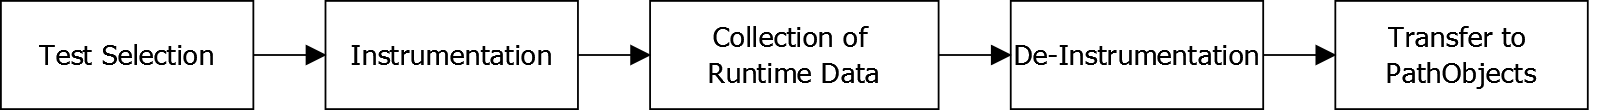
\includegraphics[width=0.9\textwidth]{../images/04-Tracing}
	\caption[TOC Caption]{Tracing foo}
	\label{fig:ImplementationTracing}
\end{figure}

\subsubsection{Shallow Analysis}

Figure \ref{fig:ImplementationTracing} depicts the fundamental steps that are performed by the \textsc{PathTools} tracing framework to generate an execution trace.
First, the user selects a test case of interest that should be traced and visualized.
For instance, this selection can be done through the list of test coverage information that is displayed next to methods in the source browser provided by the \textsc{PathTools} framework.
A \inlinecode{Tracer} object is generated which subsequently initiates the instrumentation phase.
Each method covered by the selected test case is replaced by a \inlinecode{MethodWrapper} that contains the fundamental tracing functionalities.
Thereby, only those methods are regarded that lie within the user-defined tracing scope, i.e. are a member of one of the packages the user selected for tracing.

Method wrappers \cite{brant_wrappers_1998} offer a convenient way to intercept the execution of specific methods.
As the name suggests, they wrap instances of \inlinecode{CompiledMethod} and take their place in the method dictionary of the corresponding class.
They can be utilized to execute code before and after the invocation of the wrapped method.
Furthermore, they allow the inspection and manipulation of arguments as well as of the return value of a message send.
Thereby, the operation of method wrappers is fully transparent for the callers of wrapped methods.

Afterwards, the tracer executes the specified test case.
Since all methods of interest are instrumented at this stage, they automatically report their execution to the tracer.
As method entry and exit events are recorded, a call tree of the selected test case can be constructed.

Once the execution of the test case finishes, the tracer triggers the de-instrumentation phase.
The previously created method wrappers are removed from the method dictionaries and the wrapped compiled methods are put back into their original places.

Finally, the collected information can be converted to a \textsc{PathObjects} trace, which resembles a sequential representation of the execution rather than a tree structure.

\subsubsection{Refinement Runs}
Conceptually, refinement runs are very similar to the shallow analysis process.
The differences are that no test case has to be selected, since the tracer already has a reference to the covered test case.
Furthermore, only those methods are instrumented that are actually required to collect the data that should be refined.
For instance, if the developer queries the state of an argument for a specific message send, only this method is instrumented.
Afterwards, the test is executed again and the installed method wrapper verifies if the current message send is the one the developer specified.
If this is the case, the state of this argument is recorded and reported to the tracer.
Once the test is finished, all method wrappers are removed, and the trace visualization can be updated with the refined information.

The fundamental prerequisite of this strategy is that test cases are strictly deterministic (cf. Section \ref{ss:DiscussionLimitationsTestQuality}).
Otherwise, the returned information might not be related to the developer's query.
For instance, the state of a different object might be returned when a method is called with different arguments in repeated executions.
Additionally, non-deterministic branching that yields a diverging call tree could have the consequence that the refinement run never reaches the specified point of the execution.

\section{Diagram Notation}

\section{Tools}
\subsection{Navigation}
\subsection{Exploration}
\subsection{Focusing}
\subsection{Information Layers}